% !TEX program = lualatex
\documentclass[a4paper,10pt,oneside,openany]{ltjsreport}
\usepackage[margin=21mm,top=19mm,bottom=20mm]{geometry}
\usepackage[haranoaji]{luatexja-preset}
\usepackage{amsmath,amssymb,graphicx,booktabs,longtable,xcolor,float}
\usepackage[unicode,colorlinks=true,linkcolor=blue!45!black,urlcolor=blue!45!black]{hyperref}
\usepackage{caption}
\captionsetup{font=small,labelfont=bf}
\setcounter{tocdepth}{0}
\setlength{\parskip}{0.45em}
\setlength{\parindent}{1em}
\raggedbottom
\newcommand{\sourcefile}[1]{{\small\texttt{\detokenize{#1}}}}
\begin{document}


\title{\Huge 実験7\\[0.6em]\LARGE mixing依存性\\[1em]\large 一次元HubbardモデルのUHF計算}

\author{保存結果の解析レポート}\date{2026年11月2日}\maketitle

\chapter*{概要}

物理条件と反強磁性型初期密度を固定し、密度混合率 $\alpha=0.10,0.25,0.50$ を比較した。全6ケースが収束し、同じ境界条件では全エネルギーがログの小数12桁まで一致する。一方、反復回数は大幅に減る。mixingは今回、到達した物理状態を変えずに数値的な収束速度を変えた。

対象は6ケース、保存図25枚である。収束は6ケース、未収束は0ケース。本書では生成物の種類ごとに章を設け、同じ条件のOBCとPBCを並べて読む。

\tableofcontents

\chapter{計算ログ：条件と最終結果}

\sourcefile{uhf_results.txt}

\section*{計算条件と量の定義}

$L=50$、$t=1$、温度 $T=0$、外部電場なし。全エネルギーと軌道エネルギーは $t$ を単位とする。
OBCは開放端、PBCはサイト50と1も接続する周期境界である。$N_e=N_\uparrow+N_\downarrow$、$\Delta N=N_\uparrow-N_\downarrow$ と定義する。
収束判定は混合前の密度残差 $r<10^{-10}$、最大反復回数は10000である。
表の「未」は未収束の最終再評価値であり、その桁数は精度保証ではない。

\begin{center}\small\setlength{\tabcolsep}{4pt}
\begin{longtable}{lrrrr}
\toprule
条件 & $N_e$ & $\Delta N$ & $U/t$ & mixing \\ \midrule
\endhead
mixing\_010 & 50 & 0 & 4 & 0.10 \\
mixing\_025 & 50 & 0 & 4 & 0.25 \\
mixing\_050 & 50 & 0 & 4 & 0.50 \\
\bottomrule\end{longtable}\end{center}

\section*{最終エネルギー}

$E=E_{\rm kin}+E_{\rm int}$、$E_{\rm int}=U\sum_i n_{i\uparrow}n_{i\downarrow}$。全エネルギーは占有軌道固有値の単純な総和ではなく、平均場の二重計数を除いた量である。

\begin{center}\small\setlength{\tabcolsep}{4pt}
\begin{longtable}{lrrrr}
\toprule
条件/境界 & 状態 & $E$ & $E_{\rm kin}$ & $E_{\rm int}$ \\ \midrule
\endhead
mixing\_010/OBC & 収束 & -23.013070704 & -43.110712441 & 20.097641737 \\
mixing\_010/PBC & 収束 & -23.455261995 & -43.889991764 & 20.434729770 \\
mixing\_025/OBC & 収束 & -23.013070704 & -43.110712440 & 20.097641737 \\
mixing\_025/PBC & 収束 & -23.455261995 & -43.889991764 & 20.434729770 \\
mixing\_050/OBC & 収束 & -23.013070704 & -43.110712440 & 20.097641737 \\
mixing\_050/PBC & 収束 & -23.455261995 & -43.889991764 & 20.434729770 \\
\bottomrule\end{longtable}\end{center}

物理条件と反強磁性型初期密度を固定し、密度混合率 $\alpha=0.10,0.25,0.50$ を比較した。全6ケースが収束し、同じ境界条件では全エネルギーがログの小数12桁まで一致する。一方、反復回数は大幅に減る。mixingは今回、到達した物理状態を変えずに数値的な収束速度を変えた。

\section*{原資料と再利用}

出典は \sourcefile{results_vault/experiment_07/} 内の各条件/OBC・PBCのログ、CSV、PNG。\\ 補助資料は \sourcefile{experiment_conditions.md} と \sourcefile{uhf.jl}。値は保存済みの結果から採り、SCFを再実行していない。

条件名は原資料のディレクトリ名である。mixing\_025は実験2の再利用。

再利用データは独立した追加試行ではない。本書の解釈は保存された有限サイズ・UHF解の範囲に限る。

\chapter{密度CSV：電荷分布と二重占有}

\sourcefile{density_checkpoint.csv}

CSVの50サイトすべてから $q_i=n_{i\uparrow}+n_{i\downarrow}$、$m_i=n_{i\uparrow}-n_{i\downarrow}$、
$D=L^{-1}\sum_i n_{i\uparrow}n_{i\downarrow}$ を計算した。密度の各スピン成分は0以上1以下で、総和は指定した粒子数に一致することを確認した。未収束時のCSVは最後の混合密度を対角化して得た出力密度であり、固定点の密度とは限らない。

\begin{center}\small\setlength{\tabcolsep}{4pt}
\begin{longtable}{lrrrr}
\toprule
条件/境界 & 状態 & $\min q_i$ & $\max q_i$ & $D$ \\ \midrule
\endhead
mixing\_010/OBC & 収束 & 1.000000 & 1.000000 & 0.100488 \\
mixing\_010/PBC & 収束 & 1.000000 & 1.000000 & 0.102174 \\
mixing\_025/OBC & 収束 & 1.000000 & 1.000000 & 0.100488 \\
mixing\_025/PBC & 収束 & 1.000000 & 1.000000 & 0.102174 \\
mixing\_050/OBC & 収束 & 1.000000 & 1.000000 & 0.100488 \\
mixing\_050/PBC & 収束 & 1.000000 & 1.000000 & 0.102174 \\
\bottomrule\end{longtable}\end{center}

電荷密度、局所磁化、平均二重占有は表示精度内で一致する。更新式は $n^{(k+1)}=(1-\alpha)n^{(k)}+\alpha F[n^{(k)}]$ である。自己無撞着点 $F[n]=n$ 自体は $\alpha$ に依存しないが、どの固定点へ到達するかや反復の安定性は一般には変わり得る。

\chapter{SCFエネルギー：反復による変化}

\sourcefile{scf_energy.png}

混合率を上げると、最終エネルギーに近づくまでの反復数が減る。OBCは $-23.013070703721$、PBCは $-23.455261994548$ に揃う。運動項と相互作用項には約 $10^{-10}$ 程度の差が残るため、丸められた全エネルギーの一致を完全に同一の浮動小数点状態と解釈しない。

各図の横軸は反復回数、縦軸は各反復で評価した全エネルギーである。図ごとに軸範囲が異なるため、見かけの傾きだけを比較しない。最終ログ値は反復終了後の再評価であり、履歴の最終点とわずかに異なる場合がある。

\begin{center}\small\setlength{\tabcolsep}{4pt}
\begin{longtable}{lrrr}
\toprule
条件/境界 & 初回 $E$ & 最終 $E$ & 最後の履歴の $|\Delta E|$ \\ \midrule
\endhead
mixing\_010/OBC & -17.140038 & -23.013071 & $0$ \\
mixing\_010/PBC & -17.699645 & -23.455262 & $0$ \\
mixing\_025/OBC & -17.140038 & -23.013071 & $0$ \\
mixing\_025/PBC & -17.699645 & -23.455262 & $0$ \\
mixing\_050/OBC & -17.140038 & -23.013071 & $0$ \\
mixing\_050/PBC & -17.699645 & -23.455262 & $0$ \\
\bottomrule\end{longtable}\end{center}

\begin{figure}[H]\centering

\begin{minipage}{0.49\linewidth}\centering

\textbf{OBC：収束}\par

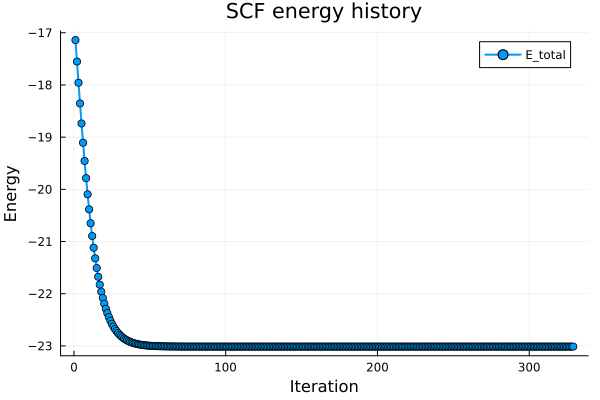
\includegraphics[width=\linewidth]{../../results_vault/experiment_07/mixing_010/OBC/scf_energy.png}

\end{minipage}\hfill%
\begin{minipage}{0.49\linewidth}\centering

\textbf{PBC：収束}\par

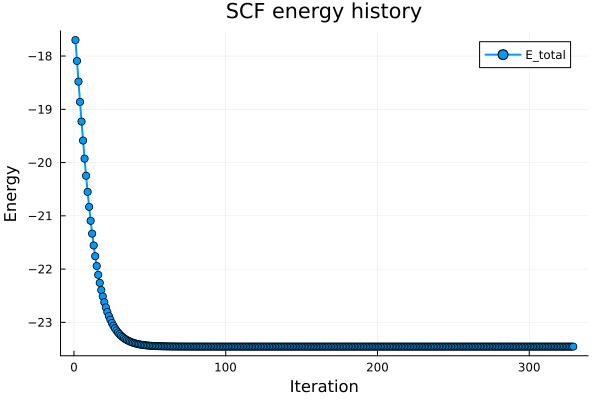
\includegraphics[width=\linewidth]{../../results_vault/experiment_07/mixing_010/PBC/scf_energy.png}

\end{minipage}

\caption{mixing\_010。SCFエネルギーの比較。左：OBC、右：PBC。}\end{figure}

\begin{figure}[H]\centering

\begin{minipage}{0.49\linewidth}\centering

\textbf{OBC：収束}\par

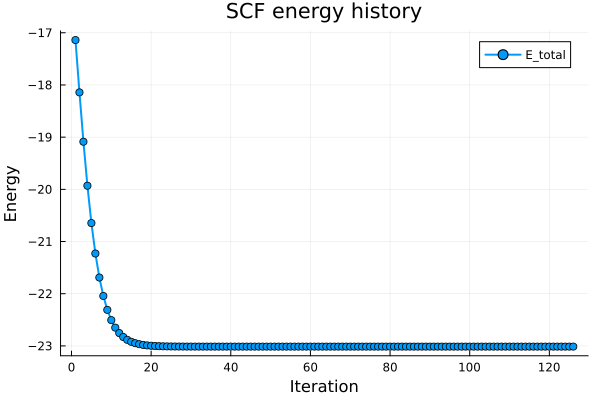
\includegraphics[width=\linewidth]{../../results_vault/experiment_07/mixing_025/OBC/scf_energy.png}

\end{minipage}\hfill%
\begin{minipage}{0.49\linewidth}\centering

\textbf{PBC：収束}\par

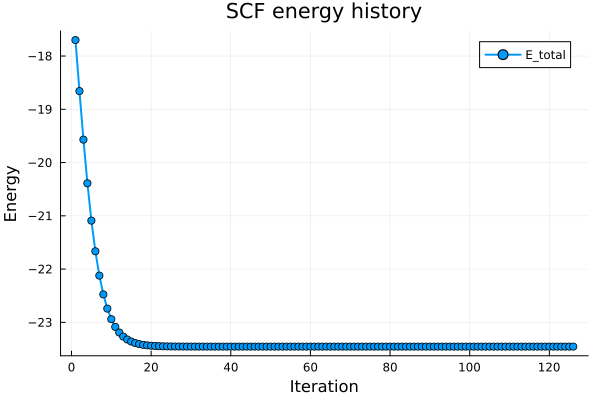
\includegraphics[width=\linewidth]{../../results_vault/experiment_07/mixing_025/PBC/scf_energy.png}

\end{minipage}

\caption{mixing\_025。SCFエネルギーの比較。左：OBC、右：PBC。}\end{figure}

\begin{figure}[H]\centering

\begin{minipage}{0.49\linewidth}\centering

\textbf{OBC：収束}\par

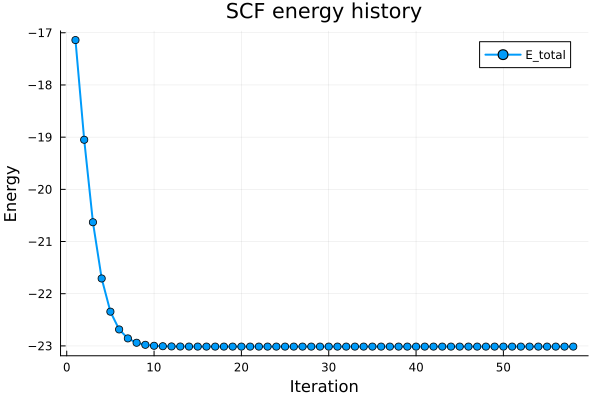
\includegraphics[width=\linewidth]{../../results_vault/experiment_07/mixing_050/OBC/scf_energy.png}

\end{minipage}\hfill%
\begin{minipage}{0.49\linewidth}\centering

\textbf{PBC：収束}\par

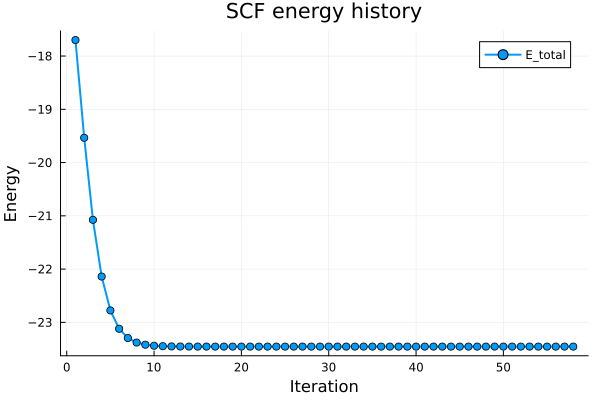
\includegraphics[width=\linewidth]{../../results_vault/experiment_07/mixing_050/PBC/scf_energy.png}

\end{minipage}

\caption{mixing\_050。SCFエネルギーの比較。左：OBC、右：PBC。}\end{figure}

\chapter{SCF残差：自己無撞着性}

\sourcefile{scf_residual.png}

反復回数は両境界条件とも329、126、58と減少する。0.10から0.50への変更で約5.67倍少ない反復で済むが、実測した実行時間の比ではない。最終残差はいずれも約 $3\times10^{-11}$ である。この範囲の半充填AF解では0.50が最速だが、未検証の混合率や他の充填・初期状態に最適値を一般化できない。

残差は $r=\max_{i,\sigma}|F[n]_{i\sigma}-n_{i\sigma}|$。表は最終再評価値である。収束時には出力密度を採用してから再評価するため、履歴図の最後の残差とは同じとは限らない。

\begin{center}\small\setlength{\tabcolsep}{4pt}
\begin{longtable}{lrrr}
\toprule
条件/境界 & 状態 & 反復数 & 最終残差 \\ \midrule
\endhead
mixing\_010/OBC & 収束 & 329 & $3.401\times10^{-11}$ \\
mixing\_010/PBC & 収束 & 329 & $3.399\times10^{-11}$ \\
mixing\_025/OBC & 収束 & 126 & $3.266\times10^{-11}$ \\
mixing\_025/PBC & 収束 & 126 & $3.263\times10^{-11}$ \\
mixing\_050/OBC & 収束 & 58 & $3.081\times10^{-11}$ \\
mixing\_050/PBC & 収束 & 58 & $3.080\times10^{-11}$ \\
\bottomrule\end{longtable}\end{center}

\begin{figure}[H]\centering

\begin{minipage}{0.49\linewidth}\centering

\textbf{OBC：収束}\par

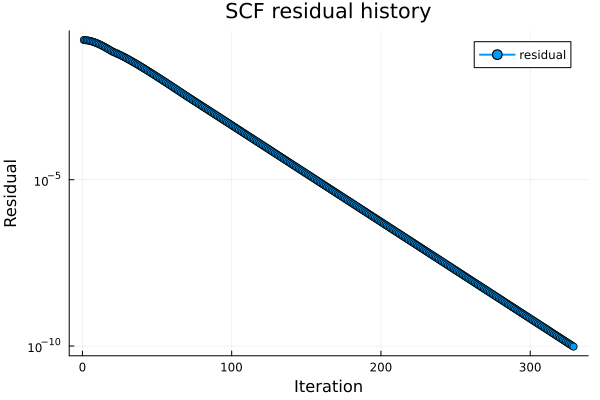
\includegraphics[width=\linewidth]{../../results_vault/experiment_07/mixing_010/OBC/scf_residual.png}

\end{minipage}\hfill%
\begin{minipage}{0.49\linewidth}\centering

\textbf{PBC：収束}\par

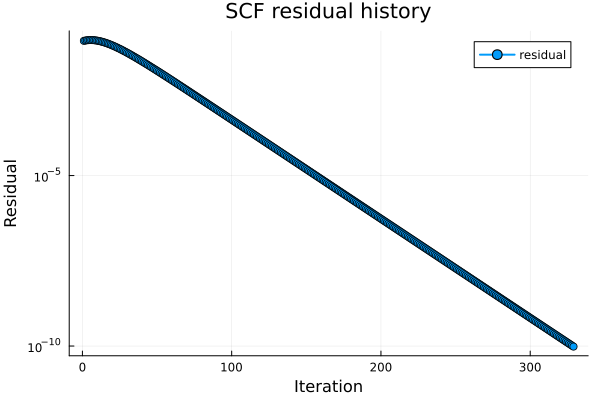
\includegraphics[width=\linewidth]{../../results_vault/experiment_07/mixing_010/PBC/scf_residual.png}

\end{minipage}

\caption{mixing\_010。SCF残差の比較。左：OBC、右：PBC。}\end{figure}

\begin{figure}[H]\centering

\begin{minipage}{0.49\linewidth}\centering

\textbf{OBC：収束}\par

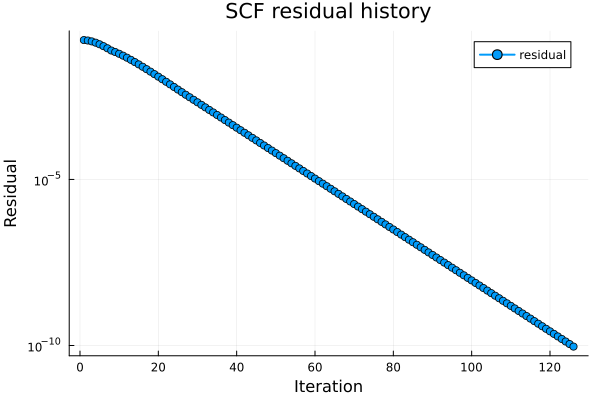
\includegraphics[width=\linewidth]{../../results_vault/experiment_07/mixing_025/OBC/scf_residual.png}

\end{minipage}\hfill%
\begin{minipage}{0.49\linewidth}\centering

\textbf{PBC：収束}\par

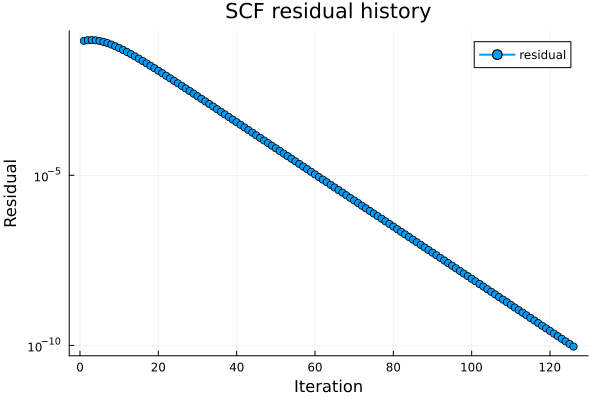
\includegraphics[width=\linewidth]{../../results_vault/experiment_07/mixing_025/PBC/scf_residual.png}

\end{minipage}

\caption{mixing\_025。SCF残差の比較。左：OBC、右：PBC。}\end{figure}

\begin{figure}[H]\centering

\begin{minipage}{0.49\linewidth}\centering

\textbf{OBC：収束}\par

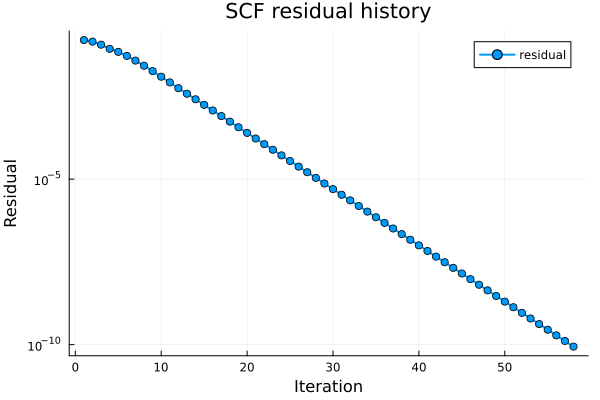
\includegraphics[width=\linewidth]{../../results_vault/experiment_07/mixing_050/OBC/scf_residual.png}

\end{minipage}\hfill%
\begin{minipage}{0.49\linewidth}\centering

\textbf{PBC：収束}\par

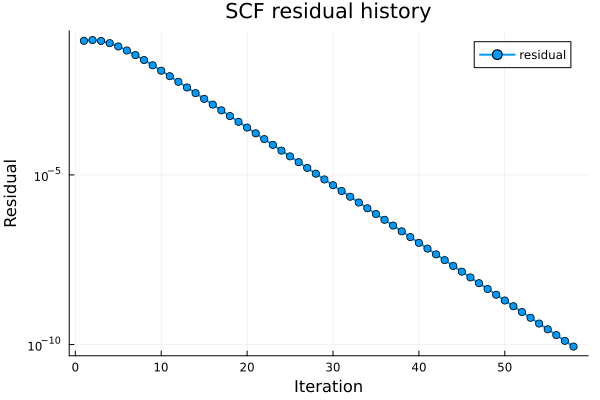
\includegraphics[width=\linewidth]{../../results_vault/experiment_07/mixing_050/PBC/scf_residual.png}

\end{minipage}

\caption{mixing\_050。SCF残差の比較。左：OBC、右：PBC。}\end{figure}

\chapter{軌道エネルギー：準位構造}

\sourcefile{final_orbital_energies.png}

各混合率の軌道固有値図は同じ形を示し、上下スピンの重なりと中央の分離が保たれる。混合率を変えても相互作用強度や粒子数は変わらないので、この一致は同じ解に到達したことを支持する。固有値の数値データは保存されておらず、図から全桁一致を主張することはできない。

横軸はエネルギー昇順の軌道番号、縦軸は $h_\sigma=h_0+U\operatorname{diag}(n_{\bar\sigma})$ の固有値である。固有値の数値ファイルは保存されていないため、図からの解釈は定性的なものに留める。未収束例をCSVから再対角化すると保存図とは異なる平均場になる可能性があり、本書ではその置換を行わない。

\begin{figure}[H]\centering

\begin{minipage}{0.49\linewidth}\centering

\textbf{OBC：収束}\par

\includegraphics[width=\linewidth]{../../results_vault/experiment_07/mixing_010/OBC/final_orbital_energies.png}

\end{minipage}\hfill%
\begin{minipage}{0.49\linewidth}\centering

\textbf{PBC：収束}\par

\includegraphics[width=\linewidth]{../../results_vault/experiment_07/mixing_010/PBC/final_orbital_energies.png}

\end{minipage}

\caption{mixing\_010。軌道エネルギーの比較。左：OBC、右：PBC。}\end{figure}

\begin{figure}[H]\centering

\begin{minipage}{0.49\linewidth}\centering

\textbf{OBC：収束}\par

\includegraphics[width=\linewidth]{../../results_vault/experiment_07/mixing_025/OBC/final_orbital_energies.png}

\end{minipage}\hfill%
\begin{minipage}{0.49\linewidth}\centering

\textbf{PBC：収束}\par

\includegraphics[width=\linewidth]{../../results_vault/experiment_07/mixing_025/PBC/final_orbital_energies.png}

\end{minipage}

\caption{mixing\_025。軌道エネルギーの比較。左：OBC、右：PBC。}\end{figure}

\begin{figure}[H]\centering

\begin{minipage}{0.49\linewidth}\centering

\textbf{OBC：収束}\par

\includegraphics[width=\linewidth]{../../results_vault/experiment_07/mixing_050/OBC/final_orbital_energies.png}

\end{minipage}\hfill%
\begin{minipage}{0.49\linewidth}\centering

\textbf{PBC：収束}\par

\includegraphics[width=\linewidth]{../../results_vault/experiment_07/mixing_050/PBC/final_orbital_energies.png}

\end{minipage}

\caption{mixing\_050。軌道エネルギーの比較。左：OBC、右：PBC。}\end{figure}

\chapter{局所磁化：空間構造}

\sourcefile{final_magnetization.png}

PBCの一様な交互磁化とOBCの端での増強は、すべての混合率で同じである。$\overline{|m|}$ はOBCで0.773051、PBCで0.768964であり、混合率による物理的な磁化変化はこの表示精度では見られない。

$\overline{|m|}=L^{-1}\sum_i|m_i|$、$M_{\rm AF}=|L^{-1}\sum_i(-1)^im_i|$ と定義する。$m_i$ はスピン密度差であり、$\langle S_i^z\rangle=m_i/2$ に対応する。全磁化は $\sum_i m_i=\Delta N$ と粒子数制約で固定される。

\begin{center}\small\setlength{\tabcolsep}{4pt}
\begin{longtable}{lrrr}
\toprule
条件/境界 & 状態 & $\overline{|m|}$ & $M_{\rm AF}$ \\ \midrule
\endhead
mixing\_010/OBC & 収束 & 0.773051 & 0.773051 \\
mixing\_010/PBC & 収束 & 0.768964 & 0.768964 \\
mixing\_025/OBC & 収束 & 0.773051 & 0.773051 \\
mixing\_025/PBC & 収束 & 0.768964 & 0.768964 \\
mixing\_050/OBC & 収束 & 0.773051 & 0.773051 \\
mixing\_050/PBC & 収束 & 0.768964 & 0.768964 \\
\bottomrule\end{longtable}\end{center}

\begin{figure}[H]\centering

\begin{minipage}{0.49\linewidth}\centering

\textbf{OBC：収束}\par

\includegraphics[width=\linewidth]{../../results_vault/experiment_07/mixing_010/OBC/final_magnetization.png}

\end{minipage}\hfill%
\begin{minipage}{0.49\linewidth}\centering

\textbf{PBC：収束}\par

\includegraphics[width=\linewidth]{../../results_vault/experiment_07/mixing_010/PBC/final_magnetization.png}

\end{minipage}

\caption{mixing\_010。局所磁化の比較。左：OBC、右：PBC。}\end{figure}

\begin{figure}[H]\centering

\begin{minipage}{0.49\linewidth}\centering

\textbf{OBC：収束}\par

\includegraphics[width=\linewidth]{../../results_vault/experiment_07/mixing_025/OBC/final_magnetization.png}

\end{minipage}\hfill%
\begin{minipage}{0.49\linewidth}\centering

\textbf{PBC：収束}\par

\includegraphics[width=\linewidth]{../../results_vault/experiment_07/mixing_025/PBC/final_magnetization.png}

\end{minipage}

\caption{mixing\_025。局所磁化の比較。左：OBC、右：PBC。}\end{figure}

\begin{figure}[H]\centering

\begin{minipage}{0.49\linewidth}\centering

\textbf{OBC：収束}\par

\includegraphics[width=\linewidth]{../../results_vault/experiment_07/mixing_050/OBC/final_magnetization.png}

\end{minipage}\hfill%
\begin{minipage}{0.49\linewidth}\centering

\textbf{PBC：収束}\par

\includegraphics[width=\linewidth]{../../results_vault/experiment_07/mixing_050/PBC/final_magnetization.png}

\end{minipage}

\caption{mixing\_050。局所磁化の比較。左：OBC、右：PBC。}\end{figure}

\chapter{境界条件による全エネルギー差}

\sourcefile{boundary_energy_difference.png}

$\Delta E_{\rm boundary}=E_{\rm PBC}-E_{\rm OBC}$ と定義する。負ならPBC、正ならOBCの保存された解の方が低エネルギーである。両方が収束した組だけを表と図で数値比較し、それ以外をNCとする。

3点とも差は $-0.442191290827$ である。境界条件によるエネルギー差が混合率変更に対して再現されたことは、今回の収束解比較の数値的な頑健性を支持する。別初期密度から得る解まで一致することを保証するものではない。

\begin{center}\small\setlength{\tabcolsep}{4pt}
\begin{longtable}{lrr}
\toprule
条件 & $\Delta E_{\rm boundary}$ & $\Delta E_{\rm boundary}/L$ \\ \midrule
\endhead
mixing\_010 & -0.442191290827 & -0.008843825817 \\
mixing\_025 & -0.442191290827 & -0.008843825817 \\
mixing\_050 & -0.442191290827 & -0.008843825817 \\
\bottomrule\end{longtable}\end{center}

\begin{figure}[H]\centering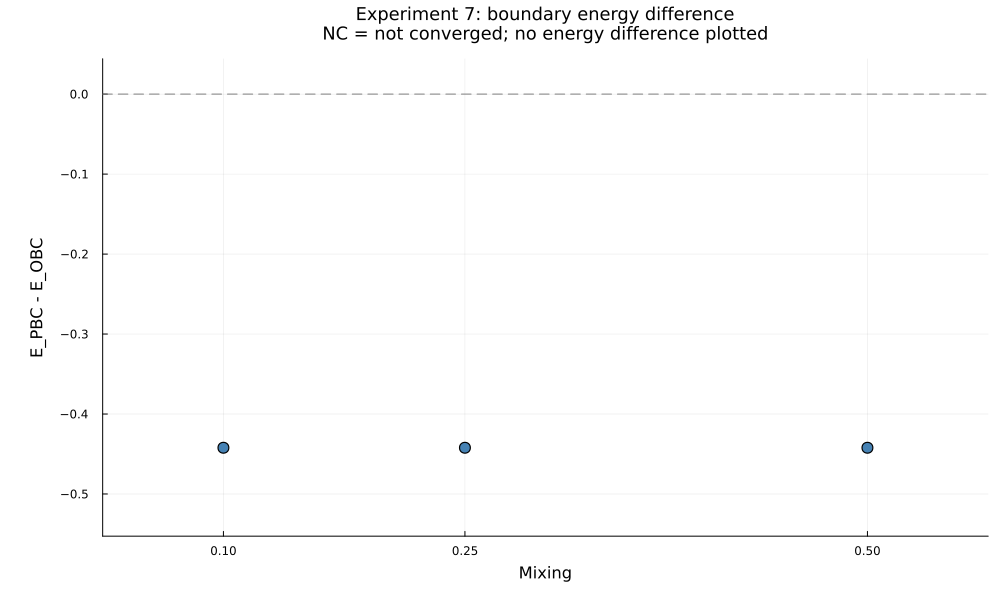
\includegraphics[width=0.9\linewidth]{../../results_vault/experiment_07/boundary_energy_difference.png}\caption{保存済みの境界エネルギー差。NCは未収束の組を示し、差が0であることを意味しない。}\end{figure}

\section*{結論と残された確認}

物理条件と反強磁性型初期密度を固定し、密度混合率 $\alpha=0.10,0.25,0.50$ を比較した。全6ケースが収束し、同じ境界条件では全エネルギーがログの小数12桁まで一致する。一方、反復回数は大幅に減る。mixingは今回、到達した物理状態を変えずに数値的な収束速度を変えた。

対象ケースはすべて収束した。ただし、収束判定だけでは得られた解が大域的な最小エネルギー状態であることまでは保証されない。

サイズは50に固定しているため、境界効果と有限サイズ効果の切り分けには別サイズの結果が必要である。

\end{document}